%{{第七十六回}}{第七十六回}}
\chapter{凸碧堂品笛感凄清\hspace{.5em}凹晶馆联诗悲寂寞}

{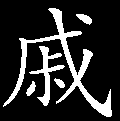
\includegraphics[width=3mm]{../Images/00005}\kaishu 此回着笔最难,不叙中秋夜宴则漏,叙夜宴又与上元相犯;不叙诸人酬和则俗,叙酬和又与起社相犯。诸人在贾政前吟诗,诸人各自为一席,又非礼。既叙夜宴再叙酬和,不漏不俗,更不相犯。云行月移,水流花放,别有机括,深宜玩索。}

话说贾赦贾政带领贾珍等散去不提。且说贾母这里命将围屏撤去,两席并而为一。众媳妇另行擦桌整果,更杯洗箸,陈设一番。贾母等都添了衣,盥漱吃茶,方又入坐,团团围绕。贾母看时,宝钗姊妹二人不在坐内,知他们家去圆月去了,且李纨凤姐二人又病着,少了四个人,便觉冷清了好些。{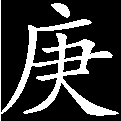
\includegraphics[width=3mm]{../Images/00004}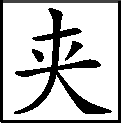
\includegraphics[width=3mm]{../Images/00012}\footnotesize \kaishu 不想这次中秋反写得十分凄楚。}贾母因笑道:``往年你老爷们不在家,咱们越性请过姨太太来,大家赏月,却十分闹热。忽一时想起你老爷来,又不免想到母子、夫妻、儿女不能一处,也都没兴。及至今年你老爷来了,正该大家团圆取乐,又不便请他们娘儿们来说说笑笑。况且他们今年又添了两口人,也难丢了他们跑到这里来。偏又把凤丫头病了,有他一人来说说笑笑,还抵得十个人的空儿。可见天下事总难十全。''说毕,不觉长叹一声,遂命拿大杯来斟热酒。王夫人笑道:``今日得母子团圆,自比往年有趣。往年娘儿们虽多,终不似今年自己骨肉齐全的好。''贾母笑道:``正是为此,所以才高兴拿大杯来吃酒。你们也换大杯才是。''邢夫人等只得换上大杯来。因夜深体乏,且不能胜酒,未免都有些倦意,无奈贾母兴犹未阑,只得陪饮。

贾母又命将罽毡铺于阶上,命将月饼、西瓜、果品等类都叫搬下去,令丫头媳妇们也都团团围坐赏月。贾母因见月至中天,比先越发精彩可爱,因说:``如此好月,不可不闻笛。''因命人将十番上女孩子传来。贾母道:``音乐多了,反失雅致,只用吹笛的远远的吹起来就够了。''说毕,刚才去吹时,只见跟邢夫人的媳妇走来向邢夫人前说了两句话。贾母便问:``说什么事?''那媳妇便回说:``方才大老爷出去,被石头绊了一下,崴了腿。''贾母听说,忙命两个婆子快看去,又命邢夫人快去。邢夫人遂告辞起身。贾母便又说:``珍哥媳妇也趁着便就家去罢,我也就睡了。''尤氏笑道:``我今日不回去了,定要和老祖宗吃一夜。''贾母笑道:``使不得,使不得。你们小夫妻家,今夜不要团圆团圆,如何为我耽搁了。''尤氏红了脸,笑道:``老祖宗说的我们太不堪了。我们虽然年轻,已经是十来年的夫妻,也奔四十岁的人了。况且孝服未满,陪着老太太顽一夜还罢了,岂有自去团圆的理。''贾母听说,笑道:``这话很是,我倒也忘了孝未满。可怜你公公已是二年多了,{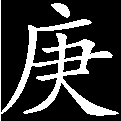
\includegraphics[width=3mm]{../Images/00004}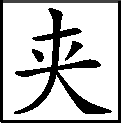
\includegraphics[width=3mm]{../Images/00012}\footnotesize \kaishu 不是算贾敬,却是算赦死期也。}可是我倒忘了,该罚我一大杯。既这样,你就越性别送,陪着我罢了。你叫蓉儿媳妇送去,就顺便回去罢。''尤氏说了。蓉妻答应着,送出邢夫人,一同至大门,各自上车回去。不在话下。

这里贾母仍带众人赏了一回桂花,又入席换暖酒来。正说着闲话,猛不防只听那壁厢桂花树下,呜呜咽咽,悠悠扬扬,吹出笛声来。趁着这明月清风,天空地净,真令人烦心顿解,万虑齐除,都肃然危坐,默默相赏。听约两盏茶时,方才止住,大家称赞不已。于是遂又斟上暖酒来。贾母笑道:``果然可听么?''众人笑道:``实在可听。我们也想不到这样,须得老太太带领着,我们也得开些心胸。''贾母道:``这还不大好,须得拣那曲谱越慢的吹来越好。''说着,便将自己吃的一个内造瓜仁油松穰月饼,又命斟一大杯热酒,送给谱笛之人,慢慢的吃了再细细的吹一套来。媳妇们答应了,方送去,只见方才瞧贾赦的两个婆子回来了,说:``右脚面上白肿了些,如今调服了药,疼的好些了,也不甚大关系。''贾母点头叹道:``我也太操心。打紧说我偏心,我反这样。''因就将方才贾赦的笑话说与王夫人尤氏等听。王夫人等因笑劝道:``这原是酒后大家说笑,不留心也是有的,岂有敢说老太太之理。老太太自当解释才是。''只见鸳鸯拿了软巾兜与大斗篷来,说:``夜深了,恐露水下来,风吹了头,须要添了这个。坐坐也该歇了。''贾母道:``偏今儿高兴,你又来催。难道我醉了不成,偏到天亮!''因命再斟酒来。一面戴上兜巾,披了斗篷,大家陪着又饮,说些笑话。只听桂花阴里,呜呜咽咽,袅袅悠悠,又发出一缕笛音来,果真比先越发凄凉。大家都寂然而坐。夜静月明,且笛声悲怨,贾母年老带酒之人,听此声音,不免有触于心,禁不住堕下泪来。众人此时都不禁凄凉寂历之意,半日,方知贾母伤感,才忙转身陪笑,发语解释。{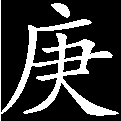
\includegraphics[width=3mm]{../Images/00004}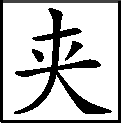
\includegraphics[width=3mm]{../Images/00012}\footnotesize \kaishu ``转身''妙!画出对月听笛如痴如呆、不觉尊长在上之形景来。}又命暖酒,且住了笛。

尤氏笑道:``我也就学一个笑话,说与老太太解解闷。''贾母勉强笑道:``这样更好,快说来我听。''尤氏乃说道:``一家子养了四个儿子:大儿子只一个眼睛,二儿子只一个耳朵,三儿子只一个鼻子眼,四儿子倒都齐全,偏又是个哑叭。''正说到这里,只见贾母已朦胧双眼,似有睡去之态。{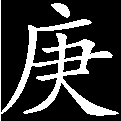
\includegraphics[width=3mm]{../Images/00004}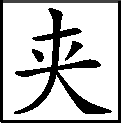
\includegraphics[width=3mm]{../Images/00012}\footnotesize \kaishu 总写出凄凉无兴景况来。}尤氏方住了,忙和王夫人轻轻的请醒。贾母睁眼笑道:``我不困,白闭闭眼养神。你们只管说,我听着呢。''{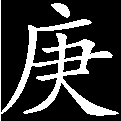
\includegraphics[width=3mm]{../Images/00004}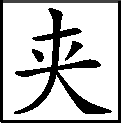
\includegraphics[width=3mm]{../Images/00012}\footnotesize \kaishu 活画。}王夫人等笑道:``夜已四更了,风露也大,请老太太安歇罢。明日再赏十六,也不辜负这月色。''贾母道:``那里就四更了?''王夫人笑道:``实已四更,他们姊妹们熬不过,都去睡了。''贾母听说,细看了一看,果然都散了,只有探春在此。贾母笑道:``也罢。你们也熬不惯,况且弱的弱,病的病,去了倒省心。只是三丫头可怜见的,尚还等着。你也去罢,我们散了。''说着,便起身,吃了一口清茶,便有预备下的竹椅小轿,便围着斗篷坐上,两个婆子搭起,众人围随出园去了。不在话下。

这里众媳妇收拾杯盘碗盏时,却少了个细茶杯,各处寻觅不见,又问众人:``必是谁失手打了。撂在那里,告诉我拿了磁瓦去交收是证见,不然又说偷起来。''众人都说:``没有打了,只怕跟姑娘的人打了,也未可知。你细想想,或问问他们去。''一语提醒了这管家伙的媳妇,因笑道:``是了,那一会记得是翠缕拿着的。我去问他。''说着便去找时,刚下了甬道,就遇见了紫鹃和翠缕来了。{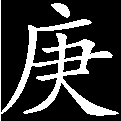
\includegraphics[width=3mm]{../Images/00004}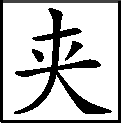
\includegraphics[width=3mm]{../Images/00012}\footnotesize \kaishu 妙!又书一个。}翠缕便问道:``老太太散了,可知我们姑娘那去了?''{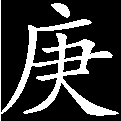
\includegraphics[width=3mm]{../Images/00004}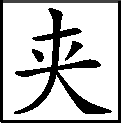
\includegraphics[width=3mm]{../Images/00012}\footnotesize \kaishu 更妙!}这媳妇道:``我来问那一个茶钟往那里去了,你们倒问我要姑娘。''翠缕笑道:``我因倒茶给姑娘吃的,展眼回头,就连姑娘也没了。''那媳妇道:``太太才说都睡觉去了。你不知那里顽去了,还不知道呢。''翠缕向紫鹃道:``断乎没有悄悄的睡去之理,只怕在那里走了一走。如今见老太太散了,赶过前边送去,也未可知。我们且往前边找找去。有了姑娘,自然你的茶钟也有了。你明日一早再找,有什么忙的。''媳妇笑道:``有了下落就不必忙了,明儿就和你要罢。''说毕回去,仍查收家伙。这里紫鹃和翠缕便往贾母处来。不在话下。

原来黛玉和湘云二人并未去睡觉。只因黛玉见贾府中许多人赏月,贾母犹叹人少,不似当年热闹,又提宝钗姊妹家去母女弟兄自去赏月等语,不觉对景感怀,自去俯栏垂泪。宝玉近因晴雯病势甚重,诸务无心,{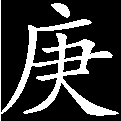
\includegraphics[width=3mm]{../Images/00004}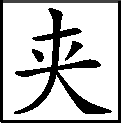
\includegraphics[width=3mm]{../Images/00012}\footnotesize \kaishu 带一笔,妙!更觉谨密不漏。}王夫人再四遣他去睡,他也便去了。探春又因近日家事着恼,无暇游玩。虽有迎春惜春二人,偏又素日不大甚合。所以只剩了湘云一人宽慰他,因说:``你是个明白人,何必作此形像自苦。我也和你一样,我就不似你这样心窄。何况你又多病,还不自己保养。可恨宝姐姐,姊妹天天说亲道热,早已说今年中秋要大家一处赏月,必要起社,大家联句,到今日便弃了咱们,自己赏月去了。社也散了,诗也不作了。倒是他们父子叔侄纵横起来。你可知宋太祖说的好:`卧榻之侧,岂许他人酣睡。'他们不作,咱们两个竟联起句来,明日羞他们一羞。''

黛玉见他这般劝慰,不肯负他的豪兴,因笑道:``你看这里这等人声嘈杂,有何诗兴。''湘云笑道:``这山上赏月虽好,终不及近水赏月更妙。你知道这山坡底下就是池沿,山坳里近水一个所在就是凹晶馆。可知当日盖这园子时就有学问。这山之高处,就叫凸碧;山之低洼近水处,就叫作凹晶。这`凸'`凹'二字,历来用的人最少。如今直用作轩馆之名,更觉新鲜,不落窠臼。可知这两处一上一下,一明一暗,一高一矮,一山一水,竟是特因玩月而设此处。有爱那山高月小的,便往这里来;有爱那皓月清波的,便往那里去。只是这两个字俗念作`洼'`拱'二音,便说俗了,不大见用,只陆放翁用了一个`凹'字,说`古砚微凹聚墨多',还有人批他俗,岂不可笑。''林黛玉道:``也不只放翁才用,古人中用者太多。如江淹《青苔赋》,东方朔《神异经》,以至《画记》上云张僧繇画一乘寺的故事,不可胜举。只是今人不知,误作俗字用了。实和你说罢,这两个字还是我拟的呢。因那年试宝玉,因他拟了几处,也有存的,也有删改的,也有尚未拟的。这是后来我们大家把这没有名色的也都拟出来了,注了出处,写了这房屋的坐落,一并带进去与大姐姐瞧了。他又带出来,命给舅舅瞧过。谁知舅舅倒喜欢起来,又说:`早知这样,那日该就叫他姊妹一并拟了,岂不有趣。'所以凡我拟的,一字不改都用了。如今就往凹晶馆去看看。''

说着,二人便同下了山坡。只一转弯,就是池沿,沿上一带竹栏相接,直通着那边藕香榭的路径。{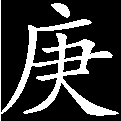
\includegraphics[width=3mm]{../Images/00004}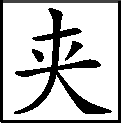
\includegraphics[width=3mm]{../Images/00012}\footnotesize \kaishu 点明,妙!不然此园竟有多大地亩了。}因这几间就在此山怀抱之中,乃凸碧山庄之退居,因洼而近水,故颜其额曰``凹晶溪馆''。因此处房宇不多,且又矮小,故只有两个老婆子上夜。今日打听得凸碧山庄的人应差,与他们无干,这两个老婆子关了月饼果品并犒赏的酒食来,二人吃得既醉且饱,早已息灯睡了。{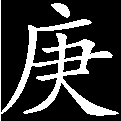
\includegraphics[width=3mm]{../Images/00004}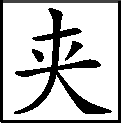
\includegraphics[width=3mm]{../Images/00012}\footnotesize \kaishu 妙极!此书有进一步写法。如王夫人云``他姊妹可怜,那里像当日林姑妈那样'',又如贾母云``如今人少,那里有当日人多''等数语,此谓进一步法也。有退一步法,如宝钗之对邢岫烟云``此一时也,彼一时也,如今比不得先的话了,只好随实守分'',又如凤姐之对平儿云``如今我也看明白了,我如今也要作好好先生罢''等类,此谓退一步法也。今又方收拾过贾母高乐,却又写出二婆子高乐,此{[}退{]}一步之实事也。如前文海棠诗四首已足,忽又用湘云独成二律反压卷,此又进一步实事也。所谓``法法皆全,丝丝不爽''也。}

黛玉湘云见息了灯,湘云笑道:``倒是他们睡了好。咱们就在这卷棚底下赏这水月如何?''二人遂在两个湘妃竹墩上坐下。只见天上一轮皓月,池中一轮水月,上下争辉,如置身于晶宫鲛室之内。微风一过,粼粼然池面皱碧铺纹,真令人神清气净。湘云笑道:``怎得这会子坐上船吃酒倒好。这要是我家里这样,我就立刻坐船了。''黛玉笑道:``正是古人常说的好,`事若求全何所乐'。据我说,这也罢了,偏要坐船起来。''湘云笑道:``得陇望蜀,人之常情。可知那些老人家说的不错。说贫穷之家自为富贵之家事事趁心,告诉他说竟不能遂心,他们不肯信的;必得亲历其境,他方知觉了。就如咱们两个,虽父母不在,然却也忝在富贵之乡,只你我竟有许多不遂心的事。''黛玉笑道:``不但你我不能趁心,就连老太太、太太以至宝玉探丫头等人,无论事大事小,有理无理,其不能各遂其心者,同一理也,何况你我旅居客寄之人哉!''{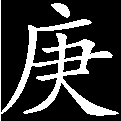
\includegraphics[width=3mm]{../Images/00004}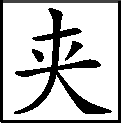
\includegraphics[width=3mm]{../Images/00012}\footnotesize \kaishu 以{(立)}{[}理{]}未{[}有{]}不怡然得享自然之乐者矣。书中若干女子从主及婢,未{(有)}必各有所觉、各有所试、各有所长者,皆未如宝{(宝)}{[}玉{]}无可关切筹划,可叹。}\href{../Text/part0080_split_000.html\#lnkback_1_a}{\textsuperscript{①}}湘云听说,恐怕黛玉又伤感起来,忙道:``休说这些闲话,咱们且联诗。''

正说间,只听笛韵悠扬起来。黛玉笑道:``今日老太太、太太高兴了,这笛子吹的有趣,倒是助咱们的兴趣了。{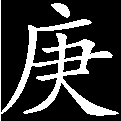
\includegraphics[width=3mm]{../Images/00004}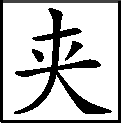
\includegraphics[width=3mm]{../Images/00012}\footnotesize \kaishu 妙!正是吹笛之时。勿认作又一处之笛也。}咱两个都爱五言,就还是五言排律罢。''湘云道:``限何韵?''黛玉笑道:``咱们数这个栏杆的直棍,这头到那头为止。他是第几根就用第几韵。若十六根,便是`一先'起。这可新鲜?''湘云笑道:``这倒别致。''于是二人起身,便从头数至尽头,止得十三根。湘云道:``偏又是`十三元'了。这韵少,作排律只怕牵强不能押韵呢。少不得你先起一句罢了。''黛玉笑道:``倒要试试咱们谁强谁弱,只是没有纸笔记。''湘云道:``不妨,明儿再写。只怕这一点聪明还有。''黛玉道:``我先起一句现成的俗语罢。''因念道:

三五中秋夕,

湘云想了一想,道:

清游拟上元。撒天箕斗灿,

林黛玉笑道:

匝地管弦繁。几处狂飞盏,

湘云笑道:``这一句`几处狂飞盏'有些意思。这倒要对的好呢。''想了一想,笑道:

谁家不启轩。轻寒风剪剪,

黛玉道:``对的比我的却好。只是底下这句又说熟话了,就该加劲说了去才是。''湘云道:``诗多韵险,也要铺陈些才是。纵有好的,且留在后头。''黛玉笑道:``到后头没有好的,我看你羞不羞。''因联道:

良夜景暄暄。争饼嘲黄发,

湘云笑道:``这句不好,是你杜撰,用俗事来难我了。''黛玉笑道:``我说你不曾见过书呢。`吃饼'是旧典,唐书唐志你看了来再说。''湘云笑道:``这也难不倒我,我也有了。''因联道:

分瓜笑绿媛。香新荣玉桂,

黛玉笑道:```分瓜'可是实实的你杜撰了。''湘云笑道:``明日咱们对查了出来大家看看,这会子别耽误工夫。''黛玉笑道:``虽如此,下句也不好,不犯着又用`玉桂'`金兰'等字样来塞责。''因联道:

色健茂金萱。蜡烛辉琼宴,

湘云笑道:```金萱'二字便宜了你,省了多少力。这样现成的韵被你得了,只是不犯着替他们颂圣去。况且下句你也是塞责了。''黛玉笑道:``你不说`玉桂',我难道强对个`金萱'么?再也要铺陈些富丽,方才是即景之实事。''湘云只得又联道:

觥筹乱绮园。分曹尊一令,

黛玉笑道:``下句好,只是难对些。''因想了一想,联道:

射覆听三宣。骰彩红成点,

湘云笑道:```三宣'有趣,竟化俗成雅了。只是下句又说上骰子。''少不得联道:

传花鼓滥喧。晴光摇院宇,

黛玉笑道:``对的却好。下句又溜了,只管拿些风月来塞责。''湘云道:``究竟没说到月上,也要点缀点缀,方不落题。''黛玉道:``且姑存之,明日再斟酌。''因联道:

素彩接乾坤。赏罚无宾主,

湘云道:``又说他们作什么,不如说咱们。''只得联道:

吟诗序仲昆。构思时倚槛,

黛玉道:``这可以入上你我了。''因联道:

拟景或依门。酒尽情犹在,

湘云说道:``是时候了。''乃联道:

更残乐已谖。渐闻语笑寂,

黛玉说道:``这时候可知一步难似一步了。''因联道:

空剩雪霜痕。阶露团朝菌,

湘云笑道:``这一句怎么押韵,让我想想。''因起身负手,想了一想,笑道:``够了,幸而想出一个字来,几乎败了。''因联道:

庭烟敛夕棔。秋湍泻石髓,

黛玉听了,不禁也起身叫妙,说:``这促狭鬼,果然留下好的。这会子才说`棔'字,亏你想得出。''湘云道:``\elegantpar{幸而昨日看历朝文选见了这个字,我不知是何树,因要查一查。宝姐姐说不用查,这就是如今俗叫作明开夜合的。我信不及,到底查了一查,果然不错。看来宝姐姐知道的竟多。}{多多多}''黛玉笑道:```棔'字用在此时更恰,也还罢了。只是`秋湍'一句亏你好想。只这一句,别的都要抹倒。我少不得打起精神来对一句,只是再不能似这一句了。''因想了一想,道:

风叶聚云根。宝婺情孤洁,

湘云道:``这对的也还好。只是下一句你也溜了,幸而是景中情,不单用`宝婺'来塞责。''因联道:

银蟾气吐吞。药经灵兔捣,

黛玉不语点头,半日随念道:

人向广寒奔。犯斗邀牛女,

湘云也望月点首,联道:

乘槎待帝孙。虚盈轮莫定,

黛玉笑道:``又用比兴了。''因联道:

晦朔魄空存。壶漏声将涸,

湘云方欲联时,黛玉指池中黑影与湘云看道:``你看那河里怎么像个人在黑影里去了,敢是个鬼罢?''湘云笑道:``可是又见鬼了。我是不怕鬼的,等我打他一下。''因弯腰拾了一块小石片向那池中打去,只听打得水响,一个大圆圈将月影荡散复聚者几次。{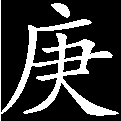
\includegraphics[width=3mm]{../Images/00004}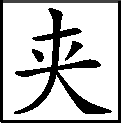
\includegraphics[width=3mm]{../Images/00012}\footnotesize \kaishu 写得出。试思若非亲历其境者如何摹写得如此。}只听那黑影里嘎然一声,却飞起一个大白鹤来,{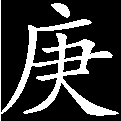
\includegraphics[width=3mm]{../Images/00004}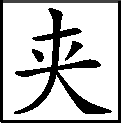
\includegraphics[width=3mm]{../Images/00012}\footnotesize \kaishu 写得出。}直往藕香榭去了。黛玉笑道:``原来是他,猛然想不到,反吓了一跳。''湘云笑道:``这个鹤有趣,倒助了我了。''因联道:

窗灯焰已昏。\elegantpar{寒塘渡鹤影}{这一联竟出在此处,早知},

林黛玉听了,又叫好,又跺足,说:``了不得,这鹤真是助他的了!这一句更比`秋湍'不同,叫我对什么才好?`影'字只有一个`魂'字可对,况且`寒塘渡鹤'何等自然,何等现成,何等有景且又新鲜,我竟要搁笔了。''湘云笑道:``大家细想就有了,不然就放着明日再联也可。''黛玉只看天,不理他,半日,猛然笑道:``你不必说嘴,我也有了,你听听。''因对道:

冷月葬花魂。\href{../Text/part0080_split_000.html\#lnkback_2_a}{\textsuperscript{②}}

湘云拍手赞道:``果然好极!非此不能对。好个`葬花魂'!''因又叹道:``诗固新奇,只是太颓丧了
些。你现病着,不该作此过于清奇诡谲之语。''黛玉笑道:``不如此,如何压倒你。下句竟还未得,只为用工在这一句了。''

一语未了,只见栏外山石后转出一个人来,笑道:``好诗,好诗,果然太悲凉了。不必再往下联,若底下只这样去,反不显这两句了,倒觉得堆砌牵强。''二人不防,倒唬了一跳。细看时,不是别人,却是妙玉。二人皆诧异,{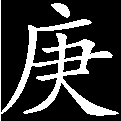
\includegraphics[width=3mm]{../Images/00004}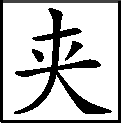
\includegraphics[width=3mm]{../Images/00012}\footnotesize \kaishu 原可诧异,余亦诧异。}因问:``你如何到了这里?''妙玉笑道:``我听见你们大家赏月,又吹的好笛,我也出来玩赏这清池皓月。顺脚走到这里,忽听见你两个联诗,更觉清雅异常,故此听住了。只是方才我听见这一首中,有几句虽好,只是过于颓败凄楚。此亦关人之气数而有,所以我出来止住。如今老太太都已早散了,满园的人想俱已睡熟了,你两个的丫头还不知在那里找你们呢。你们也不怕冷了?快同我来,到我那里去吃杯茶,只怕就天亮了。''黛玉笑道:``谁知道就这个时候了。''

三人遂一同来至栊翠庵中。只见龛焰犹青,炉香未烬。几个老嬷嬷也都睡了,只有小丫鬟在蒲团上垂头打盹。妙玉唤他起来,现去烹茶。忽听叩门之声,小丫鬟忙去开门看时,却是紫鹃翠缕与几个老嬷嬷来找他姊妹两个。进来见他们正吃茶,因都笑道:``要我们好找,一个园里走遍了,连姨太太那里都找到了。才到了那山坡底下小亭里找时,可巧那里上夜的正睡醒了。我们问他们,他们说,方才亭外头棚下两个人说话,后来又添了一个,听见说大家往庵里去。我们就知是这里了。''妙玉忙命小丫鬟引他们到那边去坐着歇息吃茶。自取了笔砚纸墨出来,将方才的诗命他二人念着,遂从头写出来。黛玉见他今日十分高兴,便笑道:``从来没见你这样高兴,\href{../Text/part0080_split_000.html\#lnkback_3_a}{\textsuperscript{③}}我也不敢唐突请教。这还可以见教否?若不堪时,便就烧了;若或可政,即请改正改正。''妙玉笑道:``也不敢妄加评赞。只是这才有了二十二韵。我意思想着你二位警句已出,再若续时,恐后力不加。我竟要续貂,又恐有玷。''黛玉从没见妙玉作过诗,今见他高兴如此,忙说:``果然如此,我们的虽不好,亦可以带好了。''妙玉道:``如今收结,到底还该归到本来面目上去。若只管丢了真情真事且去搜奇捡怪,一则失了咱们的闺阁面目,二则也与题目无涉了。''二人皆道极是。妙玉遂提笔一挥而就,递与他二人道:``休要见笑。依我必须如此,方翻转过来,虽前头有凄楚之句,亦无甚碍了。''二人接了看时,只见他续道:

香篆销金鼎,脂冰腻玉盆。

箫增嫠妇泣,衾倩侍儿温。

空帐悬文凤,闲屏掩彩鸳。

露浓苔更滑,霜重竹难扪。

犹步萦纡沼,还登寂历原。

石奇神鬼搏,木怪虎狼蹲。

赑屃朝光透,罘罳晓露屯。

振林千树鸟,啼谷一声猿。

歧熟焉忘径,泉知不问源。

钟鸣栊翠寺,鸡唱稻香村。

有兴悲何继,无愁意岂烦。

芳情只自遣,雅趣向谁言。

彻旦休云倦,烹茶更细论。

后书:右中秋夜大观园即景联句三十五韵。

黛玉湘云二人皆赞赏不已,说:``可见我们天天是舍近而求远。现有这样诗仙在此,却天天去纸上谈兵。''妙玉笑道:``明日再润色。此时想也快天亮了,到底要歇息歇息才是。''林史二人听说,便起身告辞,带领丫鬟出来。妙玉送至门外,看他们去远,方掩门进来。不在话下。

这里翠缕向湘云道:``大奶奶那里还有人等着咱们睡去呢。如今还是那里去好?''湘云笑道:``你顺路告诉他们,叫他们睡罢。我这一去未免惊动病人,不如闹林姑娘半夜去罢。''说着,大家走至潇湘馆中,有一半人已睡去。二人进去,方才卸妆宽衣,盥漱已毕,方上床安歇。紫鹃放下绡帐,移灯掩门出去。\elegantpar{谁知湘云有择席之病,虽在枕上,只白睡不着。}{认床}黛玉又是个心血不足常常失眠的,今日又错过困头,自然也是睡不着。二人在枕上翻来覆去。黛玉因问道:``怎么你还没睡着?''湘云微笑道:``我有择席的病,况且走了困,只好躺躺罢。你怎么也睡不着?''黛玉叹道:{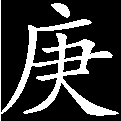
\includegraphics[width=3mm]{../Images/00004}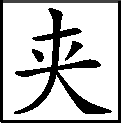
\includegraphics[width=3mm]{../Images/00012}\footnotesize \kaishu 一``笑''一``叹'',只二字便写出平日之形景。}``我这睡不着也并非今日,大约一年之中,通共也只好睡十夜满足的。''湘云道:``都是你病的原故,所以\ldots{}\ldots{}''不知下文什么------

{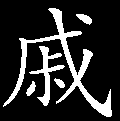
\includegraphics[width=3mm]{../Images/00005}\kaishu 总评:诗词清远闲旷,自是慧业才人,何须赘评?须看他众人联句填词时,各人性情,各人意见,叙来恰肖其人;二人联诗时,一番讥评,一番叹赏,叙来更得其神。再看漏永吟残,忽开一洞天福地,字字出人意表。}

{\kaishu 只一品笛,疑有疑无,若近若远,有无限逸致。}

% {\href{../Text/part0080_split_000.html\#navto_1_a}{①}此批非常费解。现暂以音讹校``立''为``理''(本书第五十回有``以理''二字连用例),并把一``有''字提前,意思勉强可通。是否得当,俟再推敲。曾见有其他校法,也未必是。}

% {\href{../Text/part0080_split_000.html\#navto_2_a}{②}``冷月葬花魂'',原作``冷月葬死魂'',``死''被另笔点改为``诗''。列藏、甲辰本作``冷月葬诗魂''。戚序、蒙府、杨本均作``冷月葬花魂''。``死''或以为系``花''形讹,或以为是``诗''音讹。``花魂''、``诗魂''各有出典,仔细品味,``花魂''艺术上稍胜,今从之。}

% {\href{../Text/part0080_split_000.html\#navto_3_a}{③}此后戚、蒙、列本多``若不见你这样高兴,''一句(杨本也有但又抹去)。按,有此句语意上更完足,但口语则未必会这样说。}
